\documentclass[12pt]{article}

\usepackage{sbc-template}
\usepackage{graphicx,url}
\usepackage[utf8]{inputenc}
\usepackage[brazil]{babel}
%\usepackage[latin1]{inputenc}  

     
\sloppy

\title{Perfil de desempenho e oportunidades de otimização da implementação do método CSEM 3D}

\author{Mateus F. Lima de Souza\inst{1,2}, Rômulo T. Lima\inst{1,3}, Roberto P. Souto\inst{1}, \\ 
        Antônio Tadeu A. Gomes\inst{1}, Tiziano Labruzzo\inst{1,4}, Andrea Zerilli\inst{1,4}}

\address{  Laboratório Nacional de Computação Científica (LNCC)\\
  Getúlio Vargas Av., 333, Quitandinha Petrópolis - RJ - Brasil
\nextinstitute
  Centro Federal de Educação Tecnológica Celso Suckow da Fonseca (CEFET-FR) \\
  R. Gen. Canabarro, 485 - Maracanã, Rio de Janeiro - RJ - Brasil
\nextinstitute
Universidade Católica de Petrópolis (UCP)\\
  R. Barão do Amazonas, 124 - Centro, Petrópolis - RJ - Brasil  
\nextinstitute
Zlemlink Ltda \\
Rua Taylor 39, sala 805, Rio de Janeiro-RJ - Brasil  
  \email{\{facanha,romulotl,atagomes,tiziano\}@lncc.br}
}

\begin{document} 

\maketitle

\begin{abstract}
Parallel performance profiles were obtained for one implementation of the CSEM 3D method, which is a geophysical technique used to locate oil reserves on the seabed. A routine from the PETSC library dominates the total execution time, making its efficient parallel execution result in good gain in the overall application time.
\end{abstract}
     
\begin{resumo} 
Perfis de desempenho paralelos foram obtidos para uma implementação do método CSEM 3D, que é uma técnica geofísica usada para localizar reservas de petróleo no fundo do mar. Uma rotina da biblioteca PETSC domina o tempo total de execução, fazendo com que sua execução paralela eficiente resulte em um bom ganho no tempo geral da aplicação. 
\end{resumo}


\section{Introdução}
\label{sec:intro}
%
Neste trabalho é apresentado um estudo do perfil de desempenho paralelo realizado no supercomputador Santos Dumont, de uma implementação do método CSEM-Controlled-Source Electromagnetic (método Eletromagnético de Fonte Controlada, em tradução livre)\cite{zerilli2014broadband}, que consiste em uma técnica geofísica usada para explorar o subsolo em busca de reservas de petróleo e gás, bem como de outros recursos minerais. A técnica envolve o uso de uma fonte eletromagnética para produzir um sinal de baixa frequência, que é então detectado por sensores colocados no fundo do mar. O sinal pode penetrar nas camadas do solo e interagir com qualquer material condutor, como rochas contendo hidrocarbonetos, criando um campo eletromagnético secundário que é medido pelos sensores. Ao analisar a resposta do campo secundário, pode-se criar um modelo 3D da subsolo, a ser usado para identificar a localização e o tamanho de potenciais reservas de hidrocarbonetos e outras características geológicas.

\section{Metodologia}
\label{sec:metodo}
%
A fim de obter o perfil de desempenho do CSEM 3D, foram realizadas execuções paralelas no supercomputador Santos Dumont variando-se de 12 até 384 processos MPI, usando OpenMPI v4.1.2 instalado com compilador GNU v9.3, rodado sob o pacote HPCToolkit~\cite{hpctoolkit2010}, que é um conjunto de ferramentas com código-fonte aberto para análise de desempenho, projetado para ajudar os desenvolvedores a entender e otimizar o desempenho de aplicações em sistemas de computação de alto desempenho (HPC, do termo em inglês High-Performance Computing). O HPCToolkit fornece diversos recursos para análise de desempenho, incluindo-se: \textbf{i) coleta de dados de desempenho} visando obter informações sobre o tempo de CPU, eventos de hardware, alocação de memória e outros dados relevantes para a análise de desempenho; \textbf{ii) análise de dados} para identificação dos gargalos de desempenho e oportunidades de otimização; \textbf{iii) visualização do dados} de desempenho coletados em vários formatos.


\section{Resultados}              
\label{sec:resultados}
Na Figura~\ref{fig:nodesresults} é mostrada a saída da visualização de execução paralela, respectivamente com 12 \textbf{(a)} e 384 \textbf{(b)} processos MPI. A cor azul escuro é referente ao processamento da rotina {\ttfamily \textbf{kspsolve}}, da biblioteca científica PETSC v3.18.4\cite{petsc-web-page,petsc-efficient}, que corresponde a cerca de 89\% do tempo total de execução paralela com 12 processos MPI. No entanto, com o uso de 384 processos MPI, a contribuição desta rotina da PETSC reduz-se para 35.3\%, devido justamente a boa redução de tempo alcançada pelo processamento paralelo, conforme verifica-se nas curvas de desempenho presentes na Figura~\ref{fig:desempenho}. 

%\subsection{Recursos computacionais}
\begin{figure}[hb]
\centering
\begin{tabular}{cc}
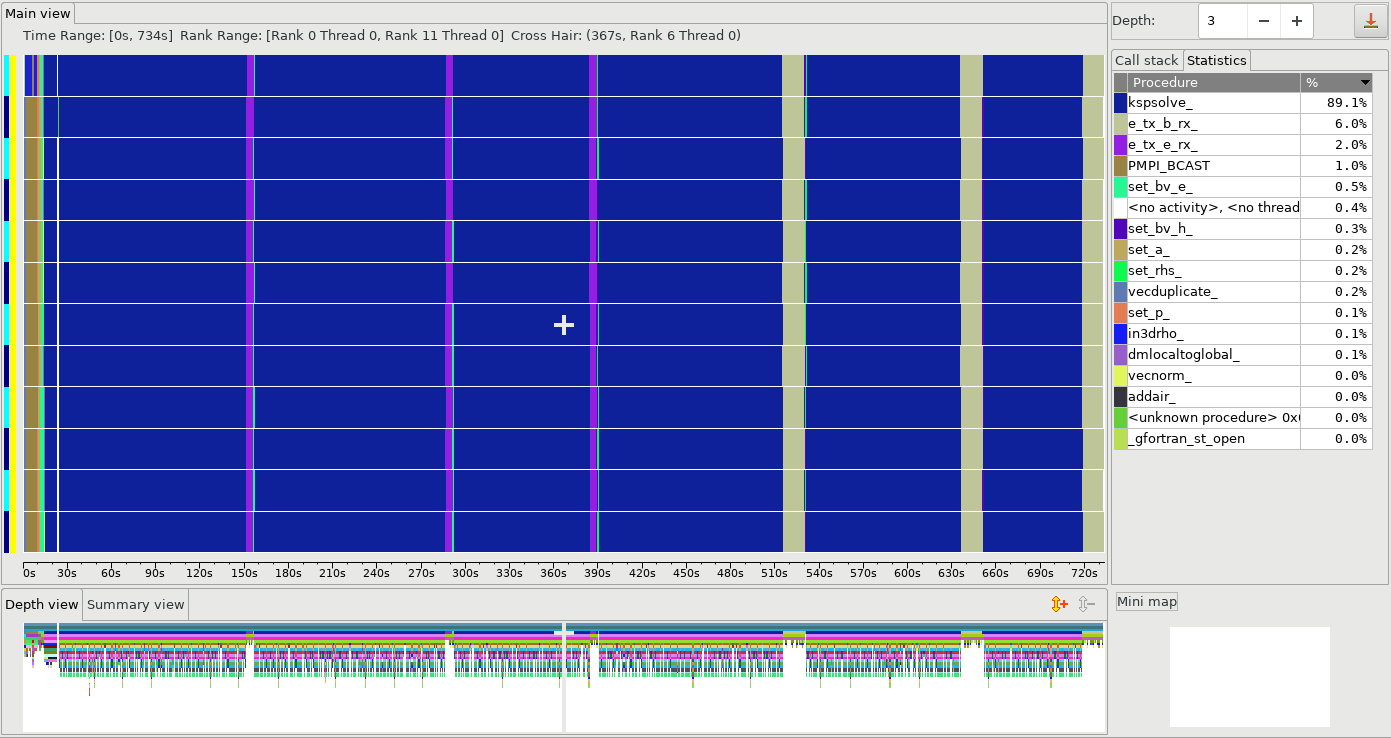
\includegraphics[width=.5\textwidth]{figures/openmpi/Nodes1_MPI12.png} & 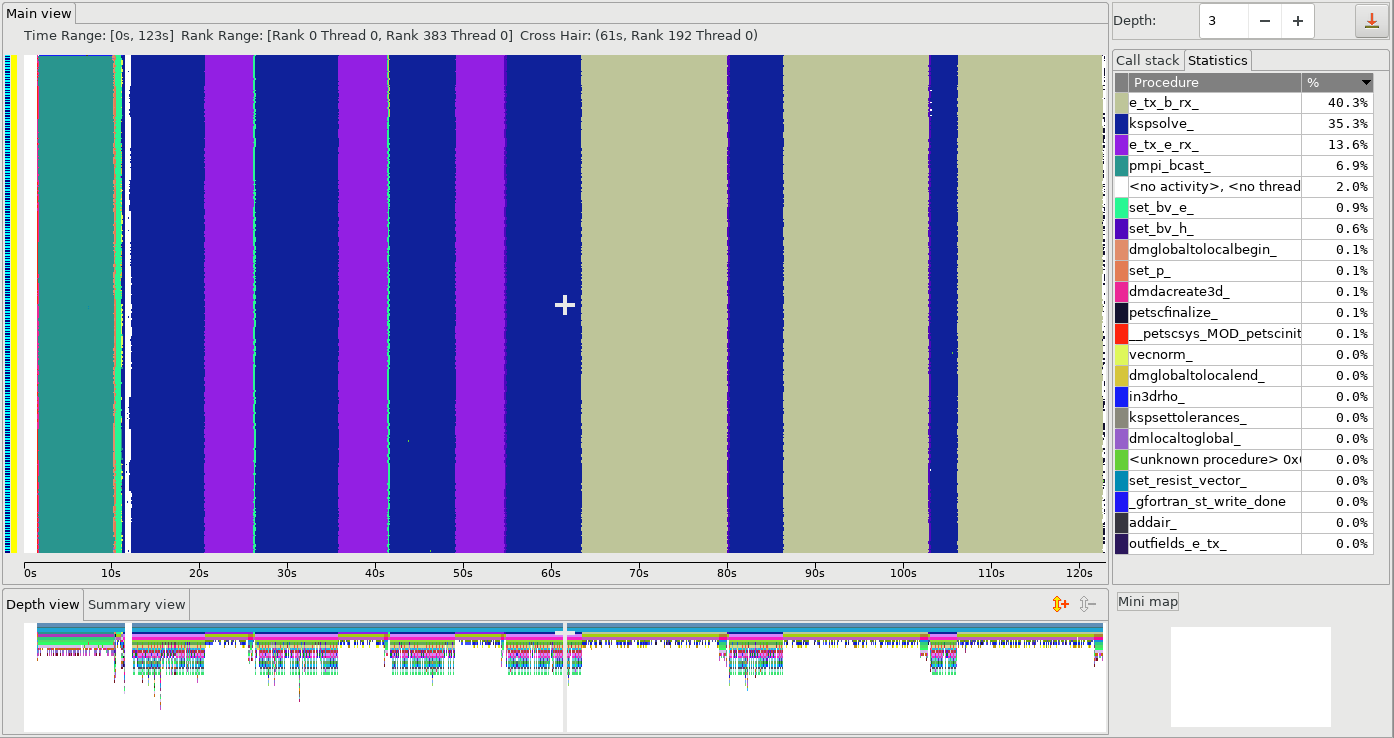
\includegraphics[width=.5\textwidth]{figures/openmpi/Nodes16_MPI384.png} \\
 \textbf{(a)} & \textbf{(b)} 
\end{tabular}
\caption{Perfis de desempenho paralelo do código CSEM 3D obtidos com o pacote HPCToolkit: com 12 \textbf{(a)} e 384 \textbf{(b)} processos MPI.}
\label{fig:nodesresults}
\end{figure}

Nota-se que praticamente toda a redução do tempo total de execução é devido ao ganho de processamento obtido pela execução paralela da rotina {\ttfamily \textbf{kspsolve}}. Portanto, é natural que a contribuição desta rotina seja proporcionalmente menor, conforme aumenta-se o número de processos MPI.

\begin{figure}[ht]
\centering
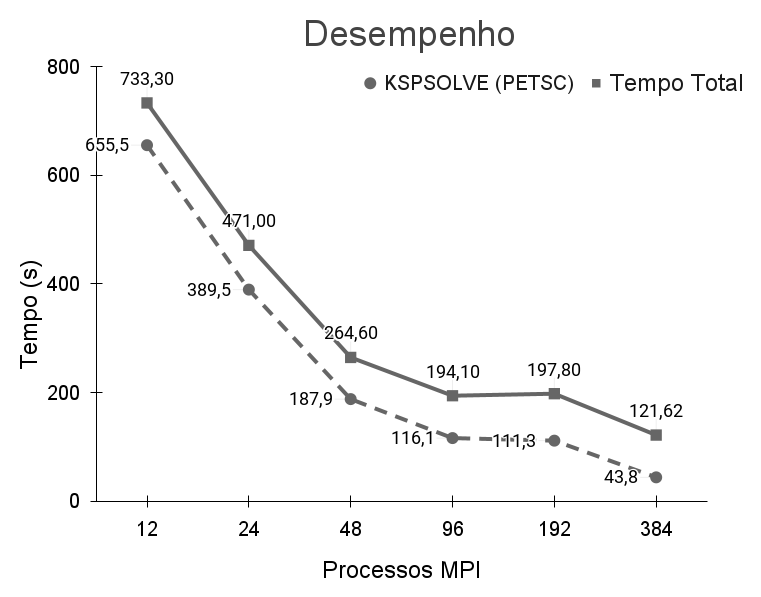
\includegraphics[width=.5\textwidth]{figures/openmpi/desempenho.png}
\caption{Curvas de desempenho paralelo de CSEM 3D (linha cheia) e somente da rotina {\ttfamily \textbf{kspsolve}} (linha tracejada) da PETSC. }
\label{fig:desempenho}
\end{figure}


\section{Comentários}
Foi apresentado um resultado inicial do desempenho paralelo do código que implementa o método CSEM 3D, onde praticamente todo ganho é obtido por uma rotina da biblioteca PETSC. Como um dos próximos passos da pesquisa, será avaliada a possibilidade de utilizar rotina da PETSC já adaptada para uso de GPU~\cite{MILLS2021}, com o quê pretende-se atingir um ganho ainda maior de desempenho.

\section*{Agradecimentos}
Os autores agradecem a Petróleo Brasileiro S.A. pelo apoio à pesquisa por meio do Termo de Colaboração número 0050.0121778.22.9. Os autores também agradecem ao Laboratório Nacional de Computação Científica (LNCC/MCTI) por fornecer recursos do supercomputador SDumont, que contribuíram para os resultados da pesquisa relatados neste artigo. \textbf{\url{http://sdumont.lncc.br}}.
%\section{References}

\bibliographystyle{sbc}
\bibliography{sbc-template}

\end{document}
